\section{Threads}

\subsection{Unterschied: Prozesse/Threads}

\begin{figure}[ht!]
    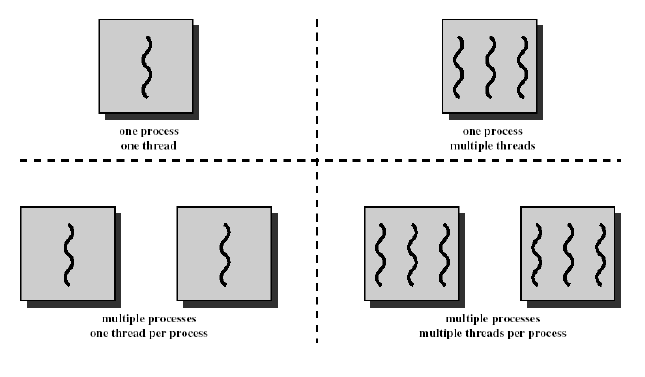
\includegraphics[width=\linewidth]{pics/processes_vs_threads}
    \caption{Unterschied zw. Prozessen und Threads}
\end{figure}

\subsection{User - und Kernel-Level Threads}

\subsubsection{User-Level Threads}
\begin{itemize}
    \item Keine Systemcalls nötig
    \item Blockiert bei I/O
    \item keine Nutzung mehrerer CPUs
    \item Bessere Abstraktion möglich
\end{itemize}

\subsubsection{Kernel-Level Threads}
\begin{itemize}
    \item BS verwalted Threads
    \item Zeitsteuerung nur mit Systemcalls
\end{itemize}

\subsubsection{Kombinierte Threadtypen}
\begin{figure}[ht!]
    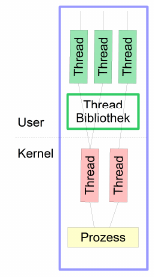
\includegraphics[scale=.8]{pics/ultklt}
    \caption{Komtiniert: ULT, KLT}
\end{figure}

\subsection{Linux Threads und Prozesse}
\textbf{Prozesse} und \textbf{Threads} werden in Linux einheitlich gehandhabt:
\begin{lstlisting}
    // Prozess
    clone(SIGCHLD, 0);
    // Thread
    clone(CLONE_VM | CLONE_FS | CLONE_FILES | CLONE_SIGHAND, 0);
\end{lstlisting}

\begin{figure}[ht!]
    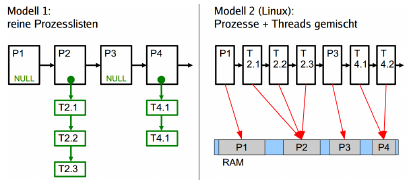
\includegraphics[scale=.8]{pics/linux_ps_th}
    \caption{Linux Prozess- und Threadverwaltung}
\end{figure}
